\section{Infrastruktur}
\label{ch:Infrastruktur}
Abbildung \vref{fig:Infrastruktur} beschreibt die Infrastruktur der Webanwendung. Entsprechend des technischen Entwurfs wurde ein Docker-Netzwerk bestehend aus mehreren Containern aufgebaut.
Die verschiedenen zusammenhängenden Services, welche in dem Netzwerk laufen sollen, werden mithilfe von \textit{Docker Compose} gestartet sowie orchestriert.  
In der Datei \textit{docker-compose.yaml} wird die Systemumgebung aufgebaut sowie die verschiedenen Docker-Container verwaltet.

\begin{figure}[h]
	\centering 
	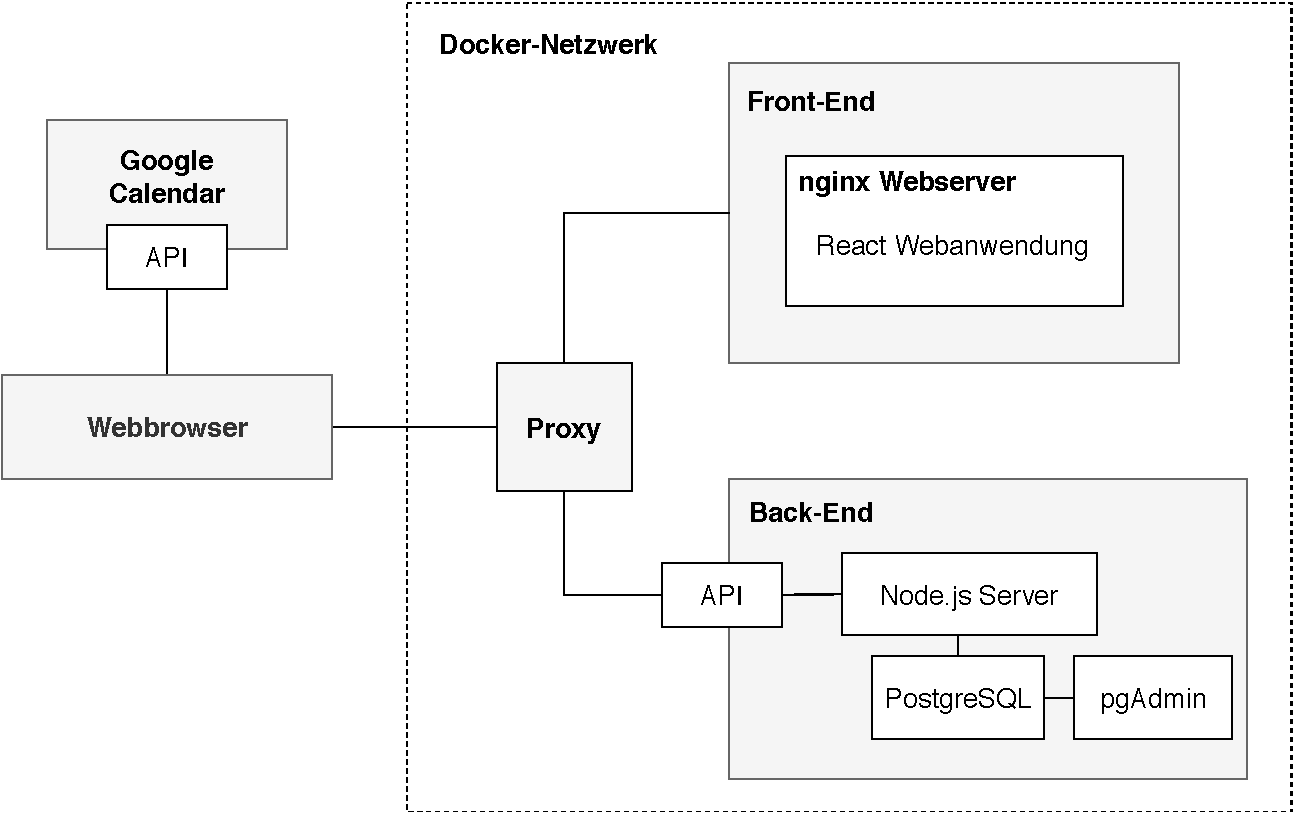
\includegraphics[width=\textwidth]{img/ImplementierungInfrastruktur.pdf}
	\caption[Übersicht der umgesetzen Infrastruktur]{\label{fig:Infrastruktur}Übersicht der umgesetzen Infrastruktur}
\end{figure}

In diesem Projekt besteht das Docker-Netzwerk aus insgesamt fünf Containern, dem Front-End-Webserver, dem Proxy, dem Back-End-Server, der Datenbank und einer graphischen Oberfläche für die Datenbank.
Durch die Verwendung von je einem Container pro Bestandteil der Infrastruktur, sind diese voneinander gekapselt und es entsteht eine verbesserte Wartbarkeit.
Einzelne Bestandteile können ziemlich einfach ausgetauscht werden, entweder durch eine andere Technologie oder für die Zeit der Wartung eines Servers.
Aber auch für die verteilte Softwareentwicklung stellt die Containerisierung einen großen Vorteil dar. 

Für das Front-End wurde ein nginx-Webserver für die Entwicklung einer Webanwendung mit React verwendet.
Das Back-End besteht aus einem Node.js-Server, welcher die Logik enthält.
Ein weiterer Bestandteil ist die PostgreSQL zur Datenhaltung in Verbindung mit pgAdmin als graphische Oberfläche zur Administration der Datenbank. 

Als zentrale Schnittstelle für die Kommunikation mit der Anwendung wird ein Proxy verwendet, welcher über einen nginx-Webserver realisiert ist.
Die Kommunikation außerhalb des Netzwerks mit dem Proxy findet verschlüsselt statt.
Aktuell werden für \acs{HTTPS} selbstsignierte Zertifikate verwendet, die vor dem Einsatz ersetzt werden müssen.
Durch den Proxy, welcher alle Anfragen von außen entgegennimmt und anschließend weiterleitet, kann die Kommunikation innerhalb des Netzwerks unverschlüsselt mit \acs{HTTP} erfolgen.
Webbrowser und der Google Calendar wurden wie in Kapitel \ref{ch:grundlegendeArchitektur} umgesetzt.

\subsubsection{GitHub}
Für die Versionsverwaltung während der Softwareentwicklung sowie das kollaborative Zusammenarbeiten wurden gemäß der logischen Trennung der Infrastruktur zwei GitHub-Repositories, für die Front-End- sowie die Back-End-Entwicklung, erstellt.
Das Back-End-Repository umfasst die Entwicklung der Geschäftslogik zusammen mit den Datenbankzugriffen und den bereitgestellten \ac{API}s.
Die Entwicklung der Benutzeroberfläche findet im Front-End-Repository statt.
Zusätzlich wurde ein GitHub-Repository für die Erstellung der Dokumentation des Projekts angelegt, welche in LaTeX verfasst wurde.
